\documentclass[12pt]{article}
\usepackage{multicol}
\usepackage{graphicx}
\usepackage{natbib}
\newcommand{\citeprimsec}[2]{\citep[][cited by \citealp{#2}]{#1}}
\usepackage{amsmath}
\usepackage{tensor}
\usepackage{float}
\usepackage{multicol}
\usepackage{amssymb}
\usepackage{mathtools}
\usepackage[english]{babel}
\usepackage{siunitx}
\sisetup{detect-all}
\usepackage[a4paper,width=150mm,top=25mm,bottom=25mm]{geometry}
\numberwithin{equation}{section}

\setlength{\parskip}{\baselineskip}%
\setlength{\parindent}{0pt}%
\begin{document}

\title{Mechanical Engineering: Year One Capstone Assesment}
\date{2019/2020}
\author{University College London}
\maketitle
\begin{flushleft}
\tableofcontents

\section*{Notes}
\begin{itemize}
  \item Titles are \textbf{not} counted towards the word limit.
  \item References are counted as one word e.g. \citeprimsec{windTurbineMaterial2}{windTurbineMaterial} is counted as \textbf{one} word. This is due to the limitations of \LaTeX \ having no word count feature.
  \item The references section at the end of the document is \textbf{not} counted towards the word limit.
  \item Inline level maths,equations and subsequent words used in equations are \textbf{not} counted towards the word limit e.g. $i = \frac{\omega_{\textrm{output}}}{\omega_{\textrm{input}}}$ the words 'output' and 'input' are not counted here.
  \item Block level maths, equations and subsequent words used in equations are counted as \textbf{one} word per line.
  \item The word count for a section is displayed at the end of the last question e.g. the 'Blades' section has five questions and the word count will be displayed after the fifth question.
  \item A total word count will appear after the word count of the final discussion section.
\end{itemize}
\newpage

\section{Blades}
\subsection[Why use composites?]{For the blades of the wind turbine, composite materials are usually employed. Why is this the case? [73/90 words]}
A composite material may be employed for their favourable properties. Composites materials can have variable properties depending on their composition; yielding better fatigue strength, elasticity and corrosion resistance than an alternative e.g. an aluminium alloy. The orientation of the fibres in the composites matrix can be specifically arranged to combat stress (in this case the force of the wind on the blade), reducing the probability of failure (cracking, deformation) in the structure.

\subsection[Common composites, relative advantages.]{What common composites might be employed in this application, and what are their relative merits and benefits in comparison to each other? [125/90 words]}
The composite used is likely to be of a fiber-reinforced matrix. The fiber used is likely to be glass or carbon based. Most common are 'E-Glass' fibers, used for their stiffness, tensile and compressive strength. They are also cheaper than carbon-based fibres. However, carbon based fibres have better mechanical properties than glass based fibres. 

The matrix material is likely to be a thermoset plastic rather than a thermoplastic. The most common thermosets used are epoxy and polyester resins. Epoxy is the more expensive option but has better mechanical properties (rigidity, strength, weight). Polyester resins also have problems with shrinkage in the curing phase, which may lead to micro-cracks and porosity. This leads to polyester resins being of a lower overall quality.

\subsection[Issues with composites.]{What significant issues can you see with using composites in this engineering application? [For 
example, you could consider economic or environmental
challenges] [145/90 words]}
A common manufacturing technique to produce turbine blades is called vacuum assisted resin transfer molding. This is where fiber sheets are placed and aligned in a mold, covered in a vacuum bag and a resin injected. The resin is then left to cure \citep{VARTM}. This process may be labour intensive, incurring high cost, as the placing and direction of the fibers is a delicate process. Once a blade has been manufactured, the blade must undergo significant testing (sometimes several months), incurring more cost. If a blade is rejected from testing, the material in the blade may be difficult to extract and reuse. 

Building on reuse, recovered fibers prevent a cost barrier. In most cases, recovered fibers are more expensive than new fibers. Thus, to use them on industrial scales is difficult. However, their reuse can be found in other fields, such as cement production \citep{fiberCement}.

\subsection[Dimensionless number derivation.]{The power (W in J/s) produced by a wind turbine depends on blade length (B), the incoming wind speed (V), and air density (\(\rho\)). Derive one dimensionless number relevant to the problem using W as the dependent parameter. Use this dimensionless number to comment on the implications of doubling the blade length. [25/90 words]}
Using Buckingham Pi:
\begin{multicols}{2}
  \begin{itemize}
    \item $[W] = ML^2T^{-3}$
    \item $[B] = L$
    \item $[V] = LT^{-1}$
    \item $[\rho] = ML^{-3}$
  \end{itemize}
\end{multicols}
\begin{align}
  W &= B^a V^b \rho^c\\
  ML^2T^{-3} &= L^a L^b T^{-b} M^c L^{-3c}\\
  c = 1, b &= 3, a = 2\\
  W &= B^2 V^3 \rho
\end{align}
\begin{gather}
  k = \frac{W_1}{B^2 V^3 \rho} \textrm{ and } k = \frac{W_2}{4B^2 V^3 \rho}\\
  W_1 = \frac{W_2}{4} \\
  4W_1 = W_2
\end{gather}
From this we can see that doubling the blade length (\(B\)), quadruples the power output of the wind turbine.

\subsection[Trade-offs with longer blade.]{Considering the answer above, discuss the trade-offs associated with choosing longer blades for a turbine of a fixed height. [83/90 words]}
Naturally, choosing larger blades for a turbine of a fixed height creates a limit to how large the blades can be before the turbine’s tower cannot structurally support the weight of the blades. Hence, using larger blades requires the use of stronger materials to support their weight. Using stronger materials is more expensive to pruchase and manufacture, driving up initial costs. If the turbine cannot produce enough power to become economically viable over its lifetime, this would cause problems for the manufacturer.

Words: 451/500

\section{Gearbox (dynamics)}
\subsection[Gear ratio derivation.]{Derive a simple relationship for the gear ratio expressed as a function of number of teeth in the sun and ring gears of an epicyclic (or planetary) gear train.}
Let us define,
\begin{multicols}{2}
  \begin{itemize} 
    \item The gear ratio $i$
    \item The sun gear with subscript $S$
    \item The planet gear(s) with subscript $P$ 
    \item The ring gear with subscript $R$
    \item The carrier with subscript $C$
    \item The number of teeth $z$
    \item The modulus of the gear(s) $m$
  \end{itemize}
\end{multicols}
The diameter of a gear is $d = mz$ and for two gears to mesh, their module must be the same. Hence, we can derive
\begin{align}
  m_1 &= m_2\\
  \frac{d_1}{z_1} &= \frac{d_2}{z_2}\\
  \frac{z_2}{z_1} &= \frac{d_2}{d_1} = \frac{r_2}{r_1}
\end{align}
From Figure (\ref{SystemRadii}), we can see that a constraint on our system is,
\begin{align}
  r_R &= r_S + 2r_P
  \label{radiiRelationship}
\end{align}

\begin{figure}[H]
  \centering
  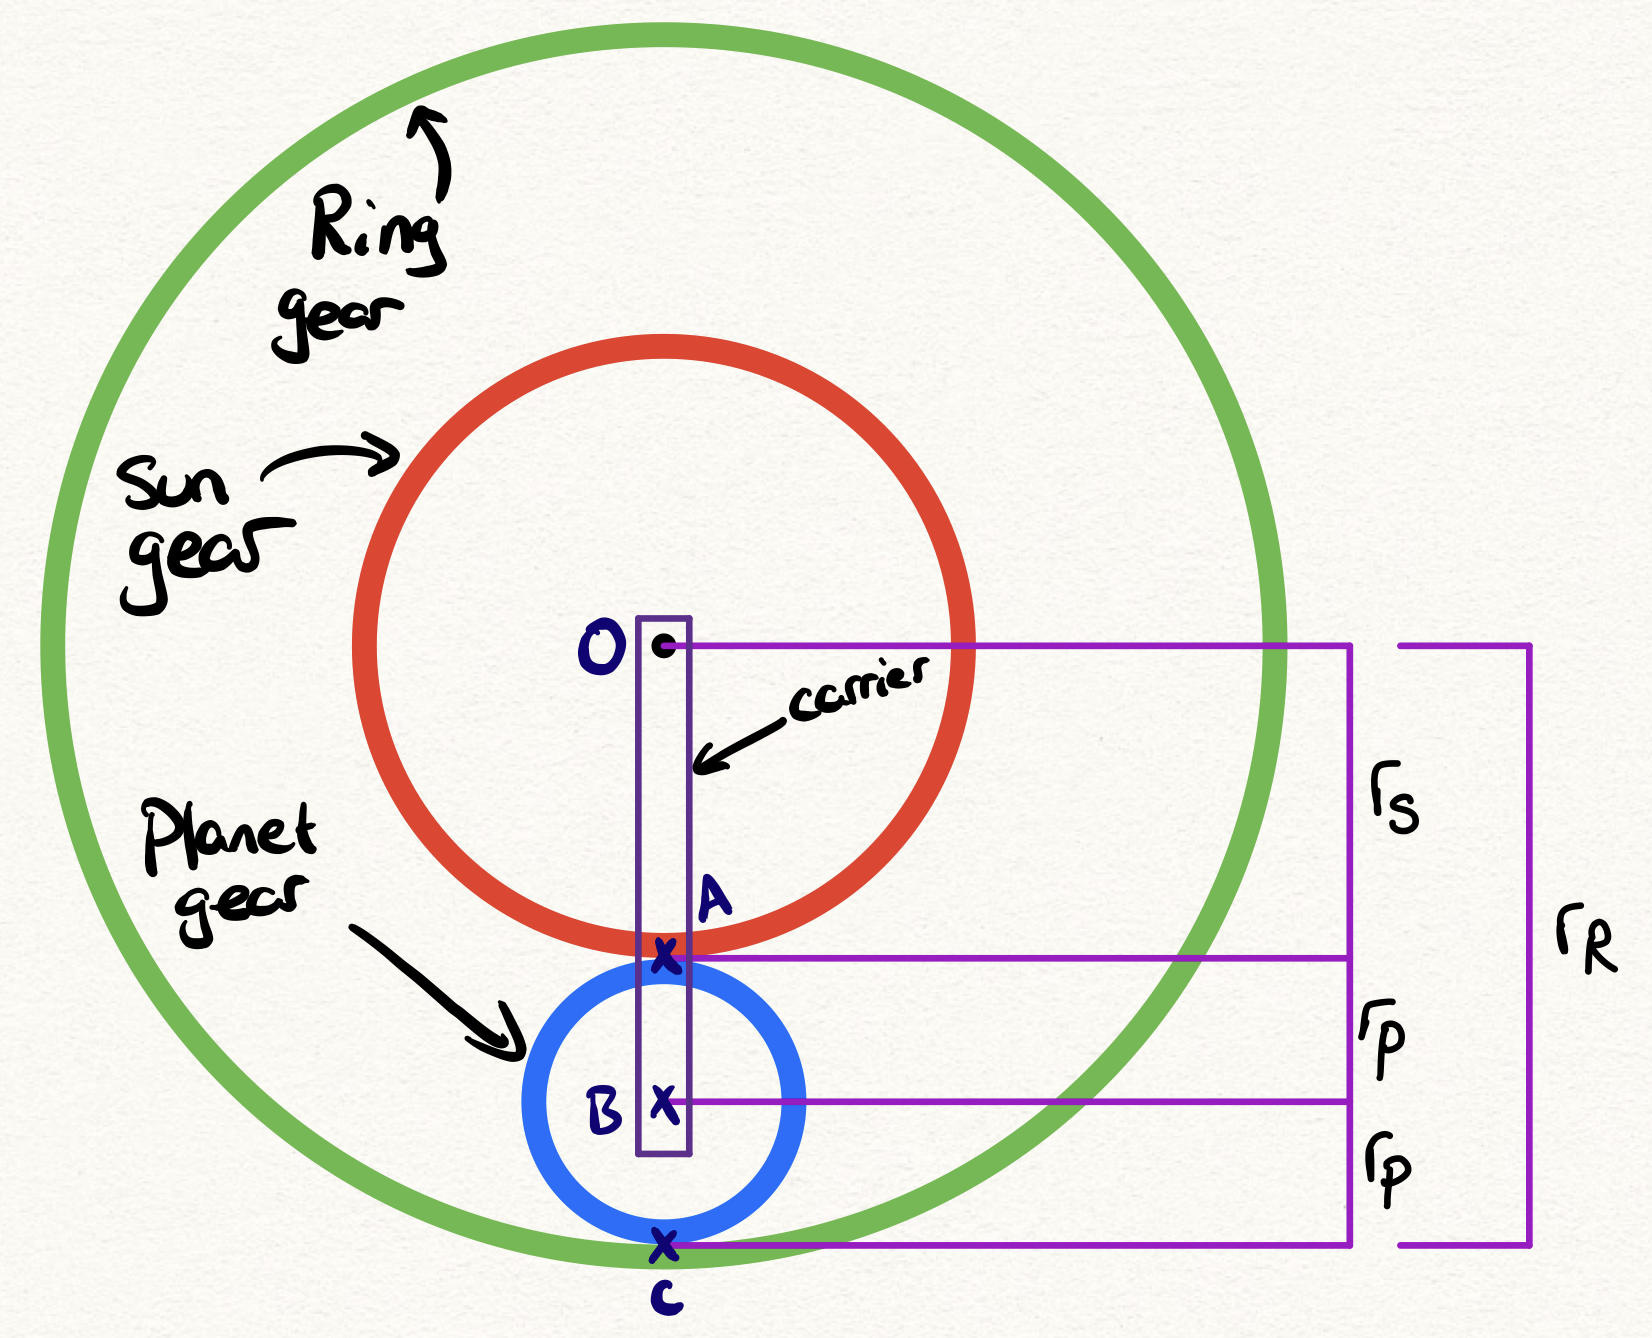
\includegraphics[width = 0.7 \textwidth]{./img/GearRadii.png}
  \caption{Simple planterary gearbox diagram.}
  \label{SystemRadii}
\end{figure}

The gear ratio of a planetary gearbox is given by the following formula.
\begin{equation}
  i = \frac{\omega_{\textrm{output}}}{\omega_{\textrm{input}}}
  \label{gearRatio}
\end{equation}
Point A experiences fixed axis rotation about centre $0$. Hence,
\begin{equation}
  v_S = \omega_S r_S
  \label{dev2Eq1}
\end{equation}
The velocity at point A can also be written as:
\begin{equation}
  v_S = v_R + v_{S/R}
\end{equation}
In the case where the ring gear is stationary, \(v_R = 0\). Subsituting this we arrive at,
\begin{equation}
  v_S = \omega_P(2r_P)
  \label{dev2Eq2}
\end{equation}
Equating equations (\ref{dev2Eq1}) and (\ref{dev2Eq2}) yields:
\begin{align}
  \omega_S r_S &= \omega_P (2r_P)\\
  \omega_P &= \frac{\omega_S r_S}{2r_P} \label{dev2Eq3}
\end{align}
Point B experience fixed axis rotation about centre $0$. Hence, 
\begin{equation}
  v_C = \omega_C r_C = \omega_C (r_S + r_P) \label{dev2Eq4}
\end{equation}
The velocity at point B can also be written as:
\begin{equation}
  v_C = v_R + v_{C/R} = 0 + r_P \omega_P \label{dev2Eq5}
\end{equation}
Using equations (\ref{dev2Eq3}), (\ref{dev2Eq4}) and (\ref{dev2Eq5}) yields:
\begin{align}
  \omega_C (r_S + r_P) &= r_P \frac{\omega_W r_S}{2r_P}\\
  \frac{\omega_S}{\omega_C} &= \frac{2(r_S + r_P)}{r_S} \label{dev2Eq6}
\end{align}
Using equation (\ref{radiiRelationship}) into (\ref{dev2Eq6}) yields:
\begin{align}
  \frac{\omega_s}{\omega_C} &= \frac{2r_S + r_R - r_S}{r_S}\\
  \frac{\omega_s}{\omega_C} &= \frac{r_S + r_R}{r_S}
\end{align}
Hence, the gear ratio $i$ is:
\begin{equation}
  i = \frac{r_S + r_R}{r_S} = 1 + \frac{r_R}{r_S}
\end{equation}
Since the number of teeth is proportional to the radius of the gear, we can substitute $z$ into our equation,
\begin{equation}
  i = 1 + \frac{z_R}{z_S}
\end{equation}
\subsection[Schematic.]{Perform a conceptual design of an epicyclic gear system for a 1.5 MW wind turbine if the three blades spin at a design speed of 12 rpm and the high-speed shaft in the generator needs to spin at 1680 rpm. Provide information on the configuration of your proposed planetary gear set (note: the 5 laws of planetary gearing – see the provided videos) and the input/output torque ratio that can be achieved by your system. Neglect friction and assume that the angular acceleration of the gears (which are rigid and non-deformable) is zero. You must indicate the number of teeth in each gear and provide a schematic drawing.}
My proposed design is to use three 4:1 planetary gearboxes with a 2.1875:1 spur gear stage. In total, $4^3 \times 2.1875 = 140$, giving us a final ratio of 140:1. This would allow the gearbox to take a 12 rpm input and convert it to 1680 rpm ($\frac{1680}{12} = 140$).

In the 4:1 planetary, the sun, planet and ring gears have teeth numbers of 29, 29, and 87 respectively. The two spur gears have teeth numbers of 35 and 16, with the 35 teeth gear being the drive gear. The torque for a planetary gearset is given by:
\begin{equation}
  \tau_S = - \tau_C \frac{N_S}{N_R + N_S}
\end{equation}
Where $\tau_S$ is the sun torque and $\tau_C$ is the carrier torque. The negative sign symbolises that output torques have the reverse sign of input torques.
Hence, after three planetaries, our torque ratio is:
\begin{align}
  \tau_{S3} &= - \tau_{C1} \left( \frac{N_S}{N_R + N_S} \right)^3\\
  \tau_{S3} &= - \tau_{C1} \left( \frac{29}{87 + 29} \right)^3\\
  \tau_{S3} &= - \frac{1}{64}\tau_{C1} 
\end{align}
For a simple gear train, the torque ratio is given by:
\begin{equation}
  R = \frac{\tau_{\textrm{driving}}}{\tau_{\textrm{driven}}}
\end{equation}
Where $R$ is the gear ratio. Hence:
\begin{align}
  \tau_{\textrm{driven}} &= \frac{\tau_{\textrm{driving}}}{R}\\
  \tau_{\textrm{driven}} &= \frac{- \frac{1}{64}\tau_{C1} }{2.1875}\\
  \tau_{\textrm{driven}} &= -\frac{1}{140} \tau_{C1}\\
  \tau_{\textrm{output}} &= -\frac{1}{140} \tau_{\textrm{input}}
\end{align}
A schematic drawing of the gearbox is shown on the next page.
\newpage
\subsection[Misalignment and failure prevention.]{Wind gusts and turbulence lead to misalignment of the drive train and premature failure of the gear components. How could this be mitigated? [124/150 words]}
Misalignment of the gear teeth can cause parts of the gear to undergo more wear and tear than normal. This abrasive action would cause more particulate matter to be generated when the gearbox is in operation. Particulate matter in the gearbox will scratch, cut and gouge material out of the gears. This can be mitigated with adequate lubrication of the gears, as it will keep the gears clean, cool and prevent a buildup of dirt and debris. 

Prevention of failure can also occur through maintenance inspections of the gearbox. A technician inspecting the gearbox will identify signs of failure in the gears and drivetrain. Components shall be replaced when needed. Processes such as cleaning can also take place to prevent further failure from occurring.

\subsection[Advantages/disadvantages of an epicyclic gearbox.]{Comment on the advantages/disadvantages of an epicyclic gear system in the context of a wind turbine gear box. [175/150 words]}
Considering that wind turbines are designed to generate power in the MWs, the gearbox must be able to withstand high torque, be small, lightweight and have great design efficiency. In an epicyclic gear system, the input load is shared between multiple planet gears. This makes them ideal for high torque use cases as the force is shared between multiple planets. Epicyclic gear systems are more space efficient than traditional gearboxes, as the driving member and the driven member are concentrically aligned. This allows multiple planetaries to be placed together in a gearbox, allowing for very high gear ratios in a small and compact size.

However, the cost to develop an epicyclic gear system is higher than a traditional gearbox. The design is more complex and because of this; it requires a higher engineering accuracy to develop the components. This design complexity also requires these gearboxes to be maintained more regularly than traditional gearboxes.

To conclude, epicyclic gear systems are a suitable fit for a wind turbine gearbox for their design efficiency and high torque capability.
\section{Gearbox (materials)}
\subsection[Why is steel used?]{For the gears in the gearbox of the wind turbine, steel would normally be the material of choice. Why is this the case? [61/150 words]}
Steel is cheap and available in a range of strengths, dependent on the carbon content. It is also tough and ductile. Steel is heat treatable and alloys with many other elements such as Chromium, Manganese and Nickel, changing its properties further. This makes steel (and its alloys) a very versatile material: easily bought and manufactured to suit the task at hand.
\subsection[What steel is suitable?]{There are many different grades of steel available – what particular properties of the steel might be required for a gearbox application, and what sorts of steel would be suitable therefore? [249/150 words]}
Let us think about the potential failures which may occur with the gears in the gearbox. Gear teeth can wear and break. Hence, we require steel with good (surface) hardness. As a side note, we may utilise lubrication to reduce the impact of shear forces on the gear. This will also help in keeping dirt and debris away from our gears, preventing misalignment and breakdown. 

The gear will be expected to have excellent longevity. On average, a wind turbine is expected to last twenty years \citep{windTurbineLifetime}. Since the wind is not a constant force, the application of forces on our gears will be cyclic. Thus the steel used should have adequate fatigue strength. The way our gear is designed will also affect this property, e.g. making sure there are no stress concentrations and making sure there is a good surface finish/contact. Manufacturing the gear this way will help reduce the potential for failure points to grow and manifest into fractures. 

We must also consider the operating conditions of our gears. Since our gearbox will be housed in the turbine's nacelle, we can assume that our gearbox will be protected from weather. The gearbox will still undergo temperature changes. Depending on the location of the wind turbine, the gears must be designed to work with the local climate in mind. Wind turbines operating in sub 20\si{\celsius} or plus 50\si{\celsius} temperatures must be designed with special considerations given to the components and infrastructure \citep{windTurbineOperatingConditions}. 

\subsection[Gearbox casing material.]{The gears will be enclosed in a housing to help hold the mechanism together and prevent the ingress of contaminants. Suggest suitable materials for this housing, ensuring you provide justification for your suggestions (taking into account a range of factors including properties, and economic issues). Given your suggestions above, qualify these by providing consideration for how such an enclosure could be manufactured. What manufacturing processes might principally be required? [153/150 words]}
A stiff and rigid material would be required to minimize vibrations from the gearbox inside. Thus, a cast metal (iron, steel or aluminium) would be a suitable fit. Cast aluminium may also be employed as it is a lighter material than cast iron/steel. Aluminium can be cast at much lower temperatures than steel and with techniques such as die casting, reducing cost. However, this also makes aluminium less heat resistant. Aluminium and stainless steel have favourable corrosion resistance properties, which is important to protect the contents from being exposed to the elements. However, stainless steel is more expensive and harder to manufacture.

To conclude, a cast aluminium casing would be the better option for a gearbox casing. Specific properties can be brought about by using a specific alloy of aluminium (such as high rigidity). The casings would be cast in two or more pieces and sealed together with rubber gaskets and bolts.

Words: 463/450

\section{Tower}
\subsection[Tower steel.]{The tower in the picture is a single tube which is also normally made of steel. Explain why this is likely to be manufactured from a different grade of steel to that used in the gearbox. What properties are needed in this particular context? [166/150 words]}
The wind turbine’s tower is expected to be a particular grade of steel because of the differing forces applied to the material. A factor to consider is how the wind force can induce an oscillation in the tower. The stiffness of the steel and natural frequency of the tower will play a dominant role in diminishing oscillations and avoiding resonance induced by the wind. A stiff steel will be more suitable in this context. 

Considering that the nacelle and blades sit atop the tower, they exhibit a compressive force on the tower. Hence, a steel with adequate compressive strength and ultimate stress to support the weight of the turbine is required. This is contrary to the steel used for the gears as they should have high tensile strength. 

Our wind turbine will again be subject to a variety of forces over its lifetime. Wind turbines are designed to have long lifespans, hence we can mitigate failure (in the material) using a high fatigue strength steel.

Words: 166/150

\section{Energy generation}
\subsection[Maximum power generation.]{Designers are considering the maximum power that could be generated by this turbine in two theoretical case studies. In case A, the incoming wind speed is 25 \si{\meter\per\second} and the air speed after passing through the blades is 15 \si{\meter\per\second}. In case B, the incoming wind speed is 20 \si{\meter\per\second} and the final speed is 12 \si{\meter\per\second}. Describe the concepts needed to estimate the maximum theoretical output of a wind turbine, and calculate the maximum theoretical power output for both these cases when the blade length is 37 \si{\meter}. Take the value of 1.2 \si{\kg\per\meter\cubed} for air density. [98/150 words]}
Power is given by:
\begin{equation}
  P = \frac{1}{4} \rho A (V_{out} + V_{in})(V_{out}^2 - V_{in}^2)
\end{equation}
\begin{itemize}
  \item $P$ = power generation in \si{\watt}.
  \item $\rho$ = density of air in \si{\kg\per\meter\cubed}.
  \item $A$ = cross section of area which a blade passes through in a revolution, measured in \si{\meter\squared}.
  \item $V_{in}$ = initial speed of wind in \si{\meter\per\second}
  \item $V_{out}$ = final speed of wind in \si{\meter\per\second}.
\end{itemize}
Our system is defined as the wind particles in the cross-sectional area of the blades.
\subsubsection*{Case A}
Variables:
\begin{multicols}{2}
  \begin{itemize}
    \item $V_{in} = 25 \ \si{\meter\per\second}$
    \item $V_{out} = 15 \ \si{\meter\per\second}$
    \item $B = 37 \ \si{\meter}$
    \item $\rho_{air} = 1.2 \ \si{\kg\per\meter\cubed}$
  \end{itemize}
\end{multicols}
Inputting the above:
\begin{gather}
  P = \frac{1}{4} \times 1.2 \times \pi \times 37^2 \times (15 + 25)(15^2 - 25^2) = -20644033.65...\\
  P = -20.6 \ \si{\mega\watt} \ (3sf)
\end{gather}
\subsubsection*{Case B}
Variables:
\begin{multicols}{2}
  \begin{itemize}
    \item $V_{in} = 20 \ \si{\meter\per\second}$
    \item $V_{out} = 12 \ \si{\meter\per\second}$
    \item $B = 37 \ \si{\meter}$
    \item $\rho_{air} = 1.2 \ \si{\kg\per\meter\cubed}$
  \end{itemize}
\end{multicols}
Inputting the above:
\begin{gather}
  P = \frac{1}{4} \times 1.2 \times \pi \times 37^2 \times (12 + 20)(12^2 - 20^2) = -10569745.23...\\
  P = -10.6 \ \si{\mega\watt} \ (3sf)
\end{gather}
Negative sign here is in reference to the direction of energy transfer. Energy is being transferred from the wind particles to the wind i.e. energy is leaving the system. 

\subsection[Terms important for wind turbine.]{Consider the various terms in the energy equation as they relate to a wind turbine. Describe briefly which terms are important for the wind turbine, and connect terms in the equation to the major sources of energy loss. Comment on the implications for wind turbine efficiency. [150/150 words]}
Energy balance equation for steady flow is:
\begin{equation}
  \dot{Q}_{in} + \dot{W}_{in} + \sum_{\substack{\text{i = all} \\ \text{inputs}}} \dot{m}_i \theta_i = \dot{Q}_{out} + \dot{W}_{out} + \sum_{\substack{\text{j = all} \\ \text{outputs}}} \dot{m}_j \theta_j 
\end{equation}
In a wind turbine, there is negligible heat in $\dot{Q}_{in}$ or work transfer in $\dot{W}_{in}$, hence:
\begin{equation}
  \sum_{\substack{\text{i = all} \\ \text{inputs}}} \dot{m}_i \theta_i =  \dot{Q}_{out} + \dot{W}_{out} + \sum_{\substack{\text{j = all} \\ \text{outputs}}} \dot{m}_j \theta_j 
\end{equation}
The thermal losses in the the system $\si{Q}_{out}$ are because of thermal losses from particle collisions (blades colliding with air particles) and inefficiencies in the gearbox (mechanical losses generating heat) and a variety of other factors such as generator efficiency etc.

$\dot{W}_{out}$ is energy transferred to the blades of the turbine from wind particles. The rotational energy of the blades increases as the kinetic energy of the wind particles decreases. $\theta$ represents the enthalpy, kinetic energy and potential energy of the wind particles. We can assume the wind particles to be travelling horizontally, thus $\Delta pe$ is negligible. When the wind particles pass through the blades, their enthalpy increases and kinetic energy decreases. 

To reach higher efficiencies, $\Delta ke$ must be maximised and $\dot{Q}_{out}$ must be minimised.
\subsection[Power value discrepancies.]{The world’s most powerful commercial wind turbine today has a blade length of 82m and is rated at 9.5 MW. Comment briefly on the reasons why the numbers calculated using your theoretical approach above are far larger than this actual capacity. [80/150 words]}
As stated above, energy generation is directly linked to the kinetic energy of the wind particles. One problem is that if there is 100\% $\Delta ke$, the particles would not move past the blades. However, there are also operational limits on components in the wind turbine such as the gearbox and the generator. These may prohibit the wind turbine to run at higher speeds. These components also have their own thermal and operational losses, further decreasing the potential power output.

\section{Energy storage}
\subsection[Compressed air storage system.]{In an offshore wind turbine facility, the excess energy generated is stored using a simple compressed air storage system. The wind turbine is mechanically coupled to a compressor that has a compression ratio of 200. The compressor takes in air from the surrounding at ambient pressure and temperature conditions (p0, T0) and performs a reversible adiabatic compression process. The output air from the compressor (at p1, T1) undergoes a reversible isobaric heat removal process using a heat exchanger in order to reduce the temperature to T0. The air is then stored in a high-pressure storage facility.}
We have two processes in this simple compressed air storage system:
\begin{itemize}
  \item Process 1 $\rightarrow$ 2: Reversible adiabtic compression (isentropic)
  \item Process 2 $\rightarrow$ 3: Reversible isobaric heat rejection
\end{itemize}

\begin{figure}[H]
  \centering
  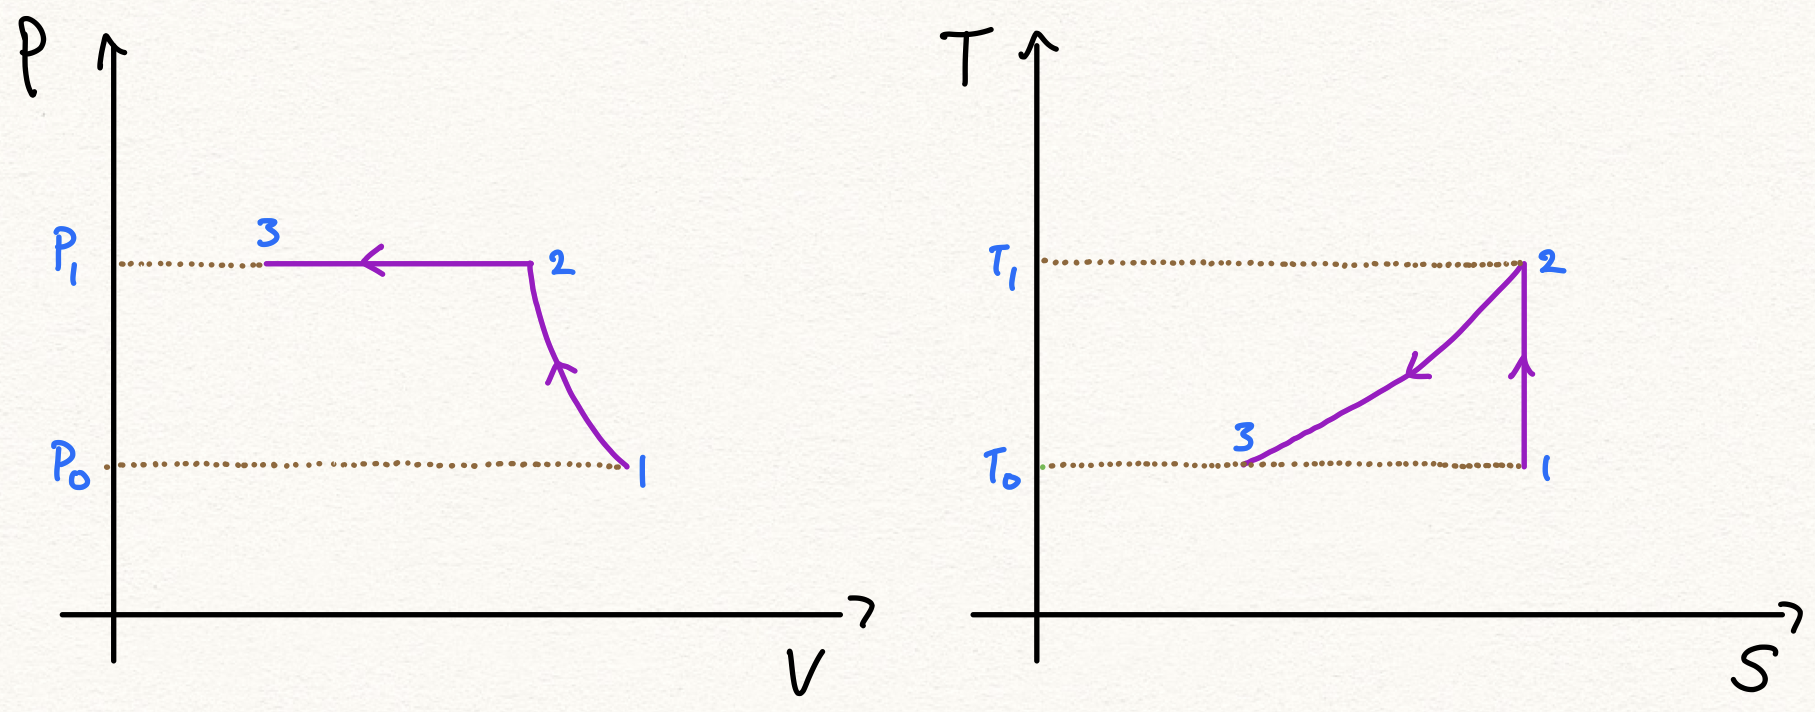
\includegraphics[width  = \textwidth]{./img/TsPvDiagrams62.png}
  \caption{Graphs to show T-s and P-v for simple compressed air storage system}
\end{figure}

\subsection{Determine:}
\subsubsection[Heat/Work transfers.]{heat and work transfers per unit mass for both the compression and heat removal processes}
\subsubsection*{Process 1 $\rightarrow$ 2: isentropic compression}
Let us begin with the First Law of Thermodynamics.
\begin{equation}
  dQ = dU + dW
\end{equation}
The process is adiabtic, hence:
\begin{align}
  dQ &= 0\\
  dW &= - dU\\
  dW &= -m c_V dT\\
  dw &= - c_V dT\\
  \int_1^2(dw) &= -c_V \int_1^2(dT)\\
  \tensor[_1]{w}{_2} &= -c_V (T_2 - T_1)\\
\end{align}
We know that $T_2 = T_1$ and $T_1 = T_0$ (as stated in question). Hence:
\begin{align}
  \tensor[_1]{w}{_2} &= -c_V (T_1 - T_0)\\
  \tensor[_1]{w}{_2} &= c_V (T_0 - T_1)
\end{align}

\subsubsection*{Process 2 $\rightarrow$ 3: reversible isobaric heat rejection}
Let us begin with the First Law of Thermodynamics.
\begin{equation}
  dQ = dU + dW
\end{equation}
Which can also be written as:
\begin{equation}
  dW = dU + PdV
\end{equation}
Assuming that ideal gas law applies, we can use the following equation. Process is isobaric, thus P is constant, as well as $n$ and $R$.
\begin{equation}
  PdV = nRdT
\end{equation}
Substituting:
\begin{equation}
  dQ = dU + nRdT
\end{equation}
$dU$ can be rewritten:
\begin{equation}
  dU = nC_V dT 
\end{equation}
Subsituting:
\begin{align}
  dQ &= nC_V dT + nRdT\\
  dQ &= ndT (C_V + R)
\end{align}
We know:
\begin{equation}
  C_P = C_V +R 
\end{equation}
Hence:
\begin{align}
  dQ &= nC_P dT\\
  dQ &= mc_P dT\\
  \int_2^3 (dQ) &= mc_P \int_2^3 (dT)\\
  \tensor[_2]{Q}{_3} &= mc_P (T_3 - T_2)
\end{align}
We know that $T_3 = T_0$ and $T_2 = T_1$ (as can be seen in the T-s diagram). Hence:
\begin{align}
  \tensor[_2]{Q}{_3} &= mc_P (T_0 - T_1)\\
  \tensor[_2]{q}{_3} &= c_P (T_0 - T_1)
\end{align}
Work done in heat rejection is simply:
\begin{align}
  \tensor[_2]{W}{_3} &= nR\int_2^3(dT)\\
  \tensor[_2]{W}{_3} &= nR(T_3 - T_2)
\end{align}
We know that $T_3 = T_0$ and $T_2 = T_1$ (as can be seen in the T-s diagram). Hence:
\begin{align}
  \tensor[_2]{W}{_3} &= nR(T_0 - T_1)\\
  \tensor[_2]{w}{_3} &= \frac{nR(T_0 - T_1)}{m}
\end{align}
\subsubsection[Entropy change.]{the total entropy change per unit mass undergone by air}
\subsubsection*{Process 1 $\rightarrow$ 2: isentropic compression}
Process is isentropic, hence:
\begin{equation}
  \tensor[_1]{s}{_2} = 0
\end{equation}
\subsubsection*{Process 2 $\rightarrow$ 3: reversible isobaric heat rejection}
Process is isobaric, hence:
\begin{align}
  dS &= \frac{dQ}{T}\\
  \int_2^3 (dS) &= \int_2^3 \left(\frac{dQ}{T} \right)\\
  \tensor[_2]{S}{_3} &= \int_2^3 \left(\frac{mc_PdT}{T}\right)\\
  \tensor[_2]{S}{_3} &= mc_P\int_2^3 \left(\frac{dT}{T}\right)\\
  \tensor[_2]{S}{_3} &= mc_P \ln \left( \frac{T_3}{T_2} \right)
\end{align}
We know that $T_3 = T_0$ and $T_2 = T_1$ (as can be seen in the T-s diagram). Hence:
\begin{align}
  \tensor[_2]{S}{_3} &= mc_P \ln \left( \frac{T_0}{T_1} \right)\\
  \tensor[_2]{s}{_3} &= c_P \ln \left( \frac{T_0}{T_1} \right)
\end{align}
Total entropy change from Process $1 \rightarrow 2 \rightarrow 3$ is:
\begin{align}
  \tensor[_1]{s}{_2} + \tensor[_2]{s}{_3} &= 0 + c_P \ln \left( \frac{T_0}{T_1} \right)\\
  \Delta s &= c_P \ln \left( \frac{T_0}{T_1} \right)
\end{align}

\subsection[SVCC Refrigerator.]{The heat removal in the above system is achieved by a refrigerator operating on a simple vapour compression cycle. This simple vapour compression refrigerator uses ammonia (NH3) as the working fluid. The evaporator pressure is pe and the condenser pressure is pc (where pc/pe>=6). The working fluid leaves the evaporator dry-saturated and enters the compressor, where it is compressed reversibly and adiabatically. Condensation at constant pressure then takes place until the saturated liquid state is reached. This is followed by throttling to evaporator pressure.}
\begin{figure}[H]
  \centering
  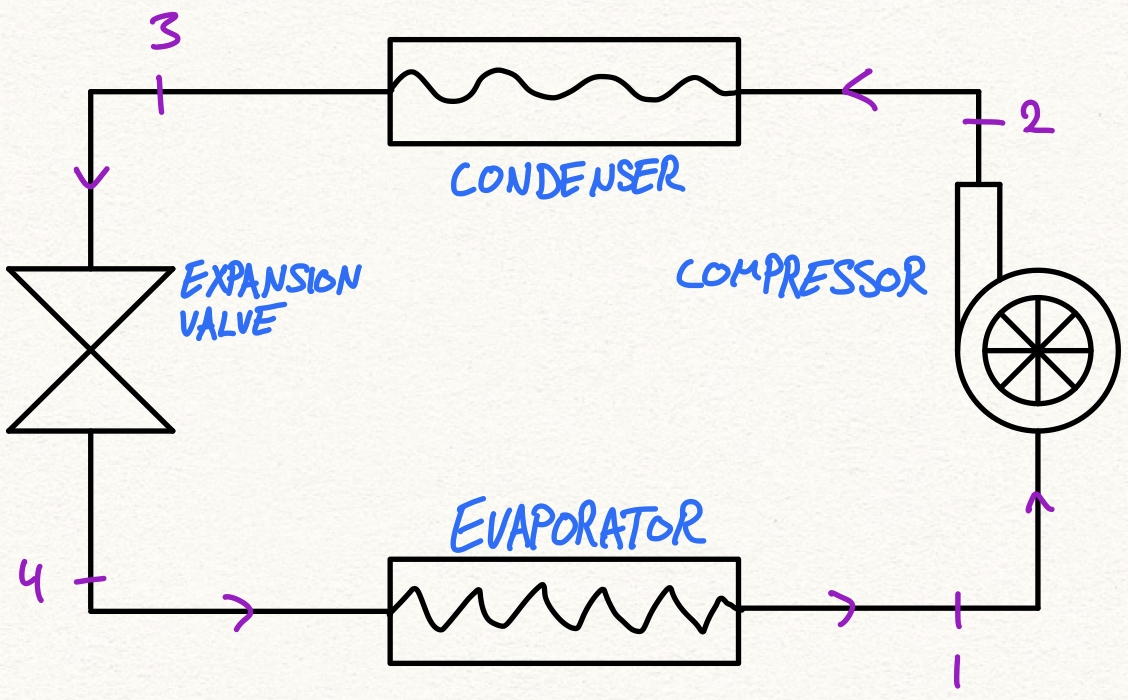
\includegraphics[width  = \textwidth]{./img/SystemDiagram63.png}
  \caption{Diagram to show simple vapour compression system}
\end{figure}
\subsection[T-s P-h Diagrams.]{Sketch the cycle on T-s and P-h diagrams}
Processes in a simple vapour compression cycle are as follows:
\begin{itemize}
  \item Process 1 $\rightarrow$ 2: Reversible adiabatic compresssion (isentropic)
  \item Process 2 $\rightarrow$ 3: Isobaric heat rejection
  \item Process 3 $\rightarrow$ 4: Thermal throttling
  \item Process 4 $\rightarrow$ 1: Isobaric heat absorption
\end{itemize}
\begin{figure}[H]
  \centering
  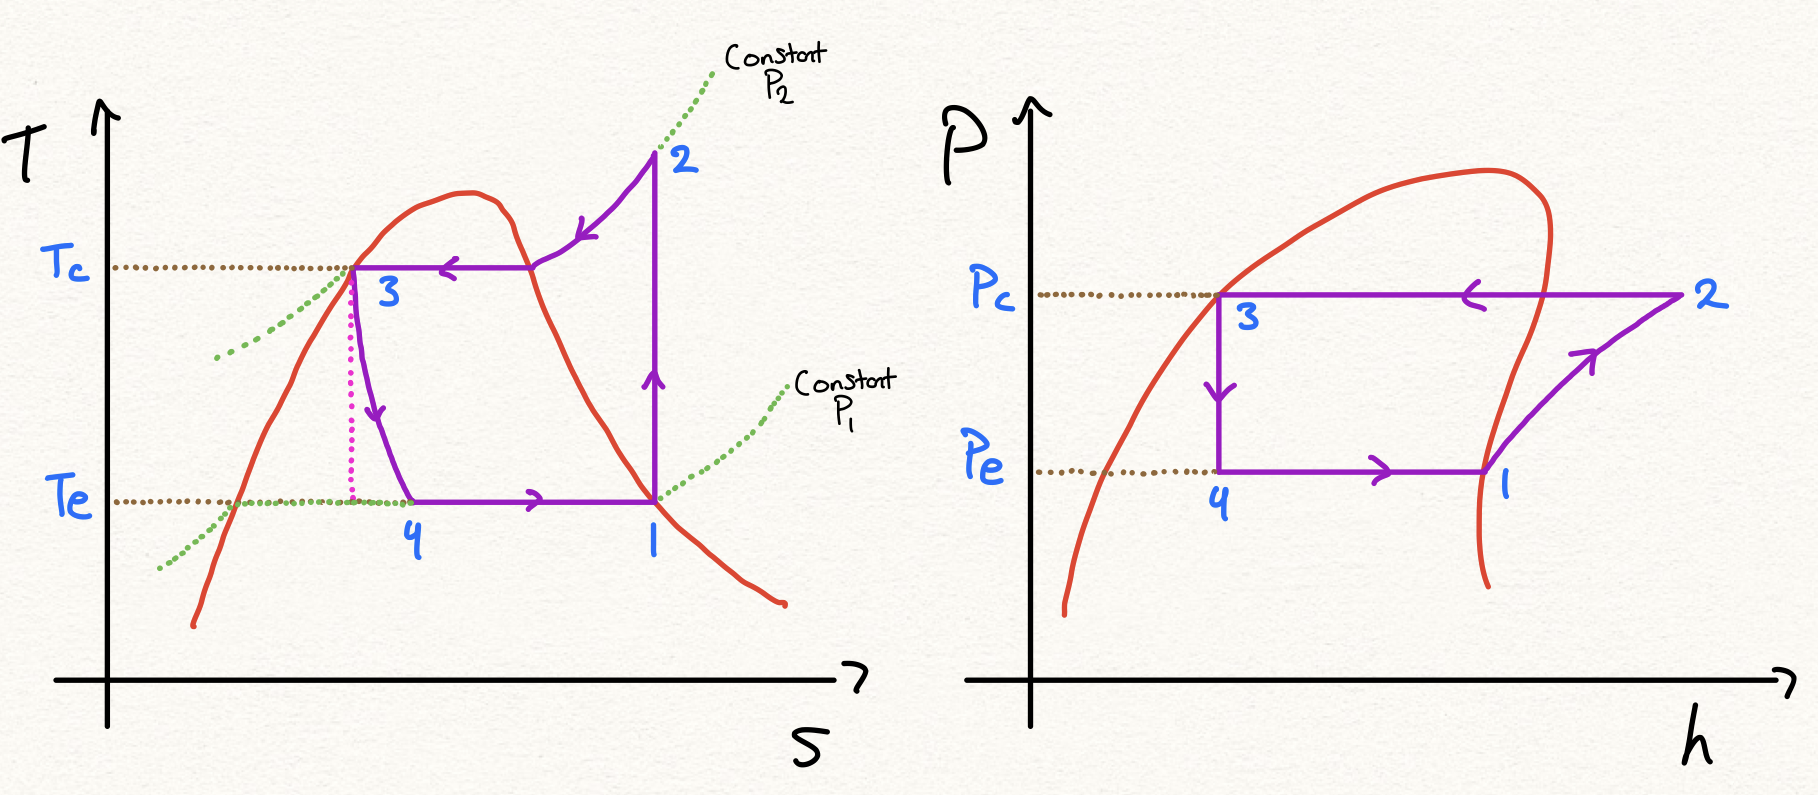
\includegraphics[width  = \textwidth]{./img/TsPhDiagrams64.png}
  \caption{Graphs to show T-s and P-h for simple vapour compression cycle}
\end{figure}
\subsection{Describe the procedure required to determine:}
\subsubsection[Compressor delivery temperature.]{the compressor delivery temperature}
Process 1 $\rightarrow$ 2 is isentropic, hence:
\begin{equation}
  s_2 = s_1 = s_{g@T_e}
\end{equation}
We can find the value for $s_2$ from thermodynamic tables for Ammonia (Refrigerant 717). We need four values from the tables:
\begin{multicols}{2}
  \begin{itemize}
    \item $s_2$
    \item $s_{T_c}$
    \item $s_{T_c + 50 \ \si{\kelvin}}$
    \item $s_{T_c + 100 \ \si{\kelvin}}$
  \end{itemize}
\end{multicols}
We need $s_{T_c + 50 \ \si{\kelvin}}$ and $s_{T_c + 100 \ \si{\kelvin}}$ for interpolation to find the temperature at $T_2$. We know that:
\begin{equation}
  s_{T_c + 50 \ \si{\kelvin}} < s_2 < s_{T_c + 100 \ \si{\kelvin}}
\end{equation}
The difference in temperature between $T_c$ and $T_2$ is $\Delta T$. Hence, using interpolation:
\begin{align}
  \frac{\Delta T - 50}{100 -50} &= \frac{s_2 - s_{T_c + 50 \ \si{\kelvin}}}{s_{T_c + 100 \ \si{\kelvin}} - s_{T_c + 50 \ \si{\kelvin}}}\\
  \Delta T &= 50 + \frac{50 \times (s_2 - s_{T_c + 50 \ \si{\kelvin}})}{s_{T_c + 100 \ \si{\kelvin}} - s_{T_c + 50 \ \si{\kelvin}}}
\end{align}
Once we have a value for $\Delta T$, we can find $T_2$ by using the following equation:
\begin{equation}
  T_2 = T_c + \Delta T
\end{equation}
\subsubsection[Refrigerant mass flow rate.]{the mass flow rate of the refrigerant}
SFEE:
\begin{multline}
  \frac{dE_{system}}{dt} = \left[ \dot{Q}_{in} + \dot{W}_{in} + \sum_{\substack{\text{i = all} \\ \text{inputs}}} \left( \dot{m}_i (h_i + \frac{v_i^2}{2} + gz_i) \right) \right] \\ - \left[ \dot{Q}_{out} + \dot{W}_{out} + \sum_{\substack{\text{j = all} \\ \text{outputs}}} \left( \dot{m}_j (h_j + \frac{v_j^2}{2} + gz_j) \right) \right]
  \label{SFEE}
\end{multline}
\begin{itemize}
  \item Neglible $\Delta KE$ and $\Delta PE$.
  \item No change in boundary volume $\therefore$ $\dot{W} = 0$
  \item No energy out $\therefore \ \dot{Q}_{out} = 0$
  \item $\dot{Q}_{in} = \dot{Q}_e$
  \item Mass flow rate of refrigerant in and out is the same $\therefore \ \dot{m}_i =\dot{m}_j = \dot{m}$
  \item $\frac{dE_{system}}{dt} = 0$
  \item $h_j = h_1 = h_{g@T_e}$
  \item $h_i = h_4 = h_3 = h_{f@T_c}$
\end{itemize}  
Simplifying equation (\ref{SFEE}), we arrive at:
\begin{align}
  0 &= \dot{Q}_{e} + 0 + \dot{m} (h_4 + 0 + 0) - \left[ 0 + 0 +  \dot{m} (h_1 + 0 + 0) \right]\\
  &= \dot{Q}_{e} + \dot{m} h_4 - \dot{m} h_1\\
  &= \dot{Q}_{e} + \dot{m} (h_4 - h_1)\\
  \dot{m} &= \frac{\dot{Q}_e}{h_1 - h_4} = \frac{\dot{Q}_e}{h_{g@T_e} - h_{f@T_c}}
\end{align}
\section{Final discussion}
\subsection*{Consider all the aspects covered above and compare the trade-offs in each of these categories during wind turbine design. You may also wish to consider how they are affected by the environment: water depth, ocean waves and seafloor structure. Reflect on the consequent additional challenges in building and maintaining offshore wind turbines.}
test

\section{scrap text}

First Process - isentropic (reverisble adiabatic) compression.
Compression ratio = 200.
Applying SFEE.
\begin{gather}
  q_{in} + w_{in} + h_0 = q_{out} + w_{out} + h_1\\
  q = 0, \ w_{out} = 0\\
  w_{in} = h_1 - h_0 \ \si{\kilo\joule\per\kg}\\
  w_{in} = c_P (T_1 - T_0)
\end{gather}
Second Process - Heat in heat removal.
Applying SFEE
\begin{gather}
  w= 0, \ q_{in} = 0\\
  q_{out} = h_2 - h_3 \ \si{\kilo\joule\per\kg}
\end{gather}
\begin{equation}
  \tensor[_1]{Q}{_2} = \tensor[_1]{q}{_2} = 0
\end{equation}
\begin{gather}
  dQ = dW + dU\\
  dQ = 0 \textrm{ (adiabtic)}\\
  dW = - dU\\
  dW = -m c_V dT
  dw = - c_V dT 
\end{gather}
\begin{gather}
  dU = -dW\\
  c_V dT = -PdV\\
  c_V dT = \frac{RT}{V} dV\\
  c_V \frac{dT}{T} = -R \frac{dV}{V}\\
  c_V\int_{T_0}^{T_1} \left( \frac{dT}{T} \right) = -R \int_{V_0}^{V_1} \left( \frac{dV}{V} \right)\\
  c_V \ln \left( \frac{T_1}{T_0} \right) = -R \ln \left( \frac{V_1}{V_0} \right) = - R \ln \left(\frac{T_1}{T_0} \frac{P_0}{P_1}\right)\\
  P_1 V_1 = R T_1\\
  V_1 = \frac{RT_1}{P_1}\\
  \therefore c_V \ln \left( \frac{T_1}{T_0} \right) = -R \ln \left(\frac{T_1}{T_0} \right) - \ln \left(\frac{P_0}{P_1}\right)\\
  (c_V + R) \ln \left(\frac{T_1}{T_0} \right) = R \ln \left(\frac{P_1}{P_0}\right)\\
  c_P \ln \left(\frac{T_1}{T_0} \right) = R \ln \left(\frac{P_1}{P_0}\right)\\
  \ln \left(\frac{T_1}{T_0} \right) = \frac{R}{c_P}\ln \left(\frac{P_1}{P_0}\right) = \ln \left(\frac{P_1}{P_0}\right)^{\frac{R}{c_P}}\\
  \frac{T_1}{T_0} = \left( \frac{P_1}{P_0} \right)^{\frac{R}{c_P}}\\
\end{gather}

\begin{equation}
  \frac{\tensor[_2]{Q}{_3}}{m} = \tensor[_2]{q}{_3} = c_P (T_0 - T_1)
\end{equation}
Work in heat removal
\begin{gather}
  \tensor[_2]{W}{_3} = k \int_2^3 \frac{dV}{V^\gamma} = \frac{P_3 V_3 - P_2 V_2}{1 - \gamma} \\
  \frac{\tensor[_2]{W}{_3}}{m} = \tensor[_2]{w}{_3} = \frac{nR(T_0 - T_1)}{m}
\end{gather}
\subsubsection{the total entropy change per unit mass undergone by air}
\begin{equation}
  \tensor[_1]{s}{_2} + \tensor[_2]{s}{_3} = 0 + c_P \ln \left( \frac{T_0}{T_1} \right)
\end{equation}

\subsubsection{Derivation One}
Considering that the sun gear is connected to the input shaft and the carrier of the planet gears is connected to the output shaft, we can simply say,
\begin{equation}
  i = \frac{\omega_S}{\omega_C}
\end{equation}
The linear velocity of the carrier is,
\begin{equation}
  v_C = \omega_C (r_S + r_P)
\end{equation}
The velocity of the point of contact between the sun and the planet gear is,
\begin{equation}
  v_S = \omega_S r_S
\end{equation}
By considering the point of contact between the planet and the ring gear as having 0 relative velocity, we can derive that the point of contact between the sun and the planet is simply $2v_C$. Hence,
\begin{align}
  v_S = 2v_C &= 2\omega_C(r_S + r_P)\\
  \omega_S r_S &= 2\omega_C (r_S + r_P)\\
  \frac{\omega_S}{\omega_C} &= \frac{2(r_S + r_P)}{r_S}\\
  &= \frac{2r_S + 2r_P}{r_S} \label{gearRatio1}
\end{align}
Rearranging equation (\ref{radiiRelationship}) and substituting into (\ref{gearRatio1}), we get,
\begin{align}
  \frac{\omega_S}{\omega_C} &= \frac{2r_S + r_R - r_S}{r_S}\\
  &= \frac{r_S + r_R}{r_S}
\end{align}
This simplifies to,
\begin{equation}
  i = 1 + \frac{r_R}{r_S}
\end{equation}
Since the number of teeth is proportional to the radius of the gear, we can substitute $z$ into our equation,
\begin{equation}
  i = 1 + \frac{z_R}{z_S}
\end{equation}

\bibliographystyle{agsm}
\bibliography{references}
\end{flushleft}
\end{document}